\documentclass[aps,prb,twocolumn,superscriptaddress,floatfix,nofootinbib]{revtex4-2}

\usepackage{amsmath,amssymb}
\usepackage{graphicx}
\usepackage{bm}
\usepackage{xcolor}
\usepackage[colorlinks=true,allcolors=blue]{hyperref}

\newcommand{\NCTO}{Na$_2$Co$_2$TeO$_6$}
\newcommand{\threeQ}{3\textbf{Q}}
\newcommand{\zz}{ZZ}
\newcommand{\meV}{\,\mathrm{meV}}
\newcommand{\ueV}{\,\mu\mathrm{eV}}
\newcommand{\Jseven}{J_7}

\graphicspath{{figs/}}%
{tuned_kruger_campaign/phase_diagram_allchan/analysis/}%
{tuned_kruger_campaign/phase_diagram/analysis/}}

\begin{document}

\title{One-defect picture for long-lived optically written zigzag order in \NCTO}

\author{}
\affiliation{}

\date{\today}

\begin{abstract}
The optically written magnetic state of \NCTO{} has two apparently conflicting
signatures: the switched zigzag state lives anomalously long, implying strong
pinning, while the clean microscopic landscape near the tuned \threeQ--zigzag
competition has only a shallow kinetic barrier and gives a sharp switching
threshold.  We resolve this with one extended disorder family: a structural line
fault that locally enhances the Kitaev exchange.  The coherent mean fault pins
the written zigzag and sets the lifetime, while bond-to-bond fluctuations around
the same enhanced-$|K|$ offset broaden the optical threshold.  A converged
climbing-image GNEB path from
the pinned zigzag strip to relaxed \threeQ{} on a $36\times36$ lattice gives a
quasi-two-dimensional depinning barrier $U_{\rm pin}=21.22\meV$, while the relaxed
\threeQ{} endpoint remains lower by $24.15\meV$, so the written state is
metastable rather than the ground state.  In driven $36\times36$ trajectories with the enhanced-$|K|$ line fixed
and zero-mean Gaussian background disorder $\delta K_{\rm bg}\sim\mathcal N(0,\sigma_K)$
added to every nearest-neighbor bond, the clean pump threshold is lowered and
broadened into a seed-resolved rounded magnetic melting curve.  The result is a lean, experimentally
testable picture in which enhanced-$|K|$ structural faults explain both the long
lifetime and the rounded optical switching fraction.
\end{abstract}

\maketitle

\section{Question}

The experimental phenomenology asks for one mechanism that is strong enough to
pin an optically written zigzag state, but not so strong that zigzag simply
becomes the equilibrium phase.  In a clean near-degenerate \threeQ--zigzag model,
the optical response is a threshold switch: below threshold the system remains
\threeQ, and above threshold it writes zigzag.  That clean threshold is too sharp
to explain a continuous switched fraction across a disordered sample.  At the
same time, the measured lifetime is far too long to be explained by the clean
barrier.  The model therefore has to explain two different signatures:
\begin{enumerate}
\item a metastable written zigzag state with a large depinning barrier;
\item a disorder-broadened optical threshold, so switching appears as continuous
magnetic melting rather than an all-or-nothing clean transition.
\end{enumerate}
The central point of this note is that these two signatures can be obtained from
one microscopic imperfection family.  We use an extended enhanced-$|K|$ line as
the hard lifetime fault, and we broaden the switching threshold by adding
zero-mean Gaussian disorder to every nearest-neighbor bond.

\section{Model and observables}

The spin Hamiltonian is the extended Kitaev model on the honeycomb lattice,
\begin{equation}
\mathcal H=\mathcal H_{\rm NN}(J,K,\Gamma,\Gamma')
+\mathcal H_{2}(J_{2A},J_{2B})+\mathcal H_{3}(J_3)+\mathcal H_7,
\end{equation}
where $\mathcal H_{\rm NN}$ contains the standard bond-dependent
Kitaev-Heisenberg-$\Gamma$-$\Gamma'$ nearest-neighbor exchange.  The tuned Kruger
parameters, in meV, are
\begin{equation}
\begin{aligned}
J&=0.68, & K&=-7.89, & \Gamma&=3.07, & \Gamma'&=-2.94,\\
J_{2A}&=-0.06, & J_{2B}&=-0.70, & J_3&=0.52, & J_7&=-0.40.
\end{aligned}
\end{equation}
The ring term $J_7$ is used only as the near-degeneracy knob: at this
working point relaxed \threeQ{} remains slightly lower than zigzag, but the two
states are close enough that an $E_1$ phonon pump can switch the order.

Driven trajectories use the $E_1$ phonon protocol with Gr\"uneisen-scaled
coupling to all four nearest-neighbor exchange channels:
$\lambda_{E_1,K_2}=0.02$, $\lambda_{E_1,J_2}=0.0017$, $\lambda_{E_1,\Gamma_2}=0.0078$,
$\lambda_{E_1,\Gamma'_2}=0.0075$ (in the proportional relation
$\lambda_{E_1,X_2}=|X|/|K|\times\lambda_{E_1,K_2}$),
$\omega_{E1}=4.0$, $\gamma_{E1}=0.0849$, pump
center $50$, width $15$, Gilbert damping $\alpha=0.05$, RK4 time step
$0.005$.  All production results emphasized below use $L=36$ honeycomb lattices
($N=2592$ spins): the selected hard-fault GNEB path, the fixed-line
global-disorder switching fraction, and the regenerated defect geometry are all
evaluated on the same solver lattice convention.  With Gr\"uneisen-scaled all-channel coupling the clean fixed-line threshold lies
between $E_0=20$ and $22$ (the seed-0 trajectory is off at $E_0=20$ and fully
switched at $E_0=22$); global disorder lowers the 25\% crossing from
$E_0\simeq21$ down to $E_0\simeq10$--$14$ as $\sigma_K$ grows.  The order
diagnostic is
the ratio
\begin{equation}
r_3=\frac{\min_i S(\bm M_i)}{\max_i S(\bm M_i)},
\end{equation}
over the three zigzag wave vectors.  We also use a local zigzag overlap to count
the fraction of sites written into the targeted zigzag domain after a quench.

For kinetic barriers we use the climbing-image geodesic nudged-elastic-band
method on the curved spin manifold.  The GNEB path shown below is the physical
depinning path from the pinned zigzag strip to relaxed \threeQ{} with the defect
present.  The energy zero is the pinned zigzag endpoint; the right endpoint is
the relaxed \threeQ{} state.  Thus a negative final endpoint in the plot means
that \threeQ{} is lower in energy and the written zigzag state is metastable.

\section{Clean switching landscape}

\begin{figure}[t]
\centering
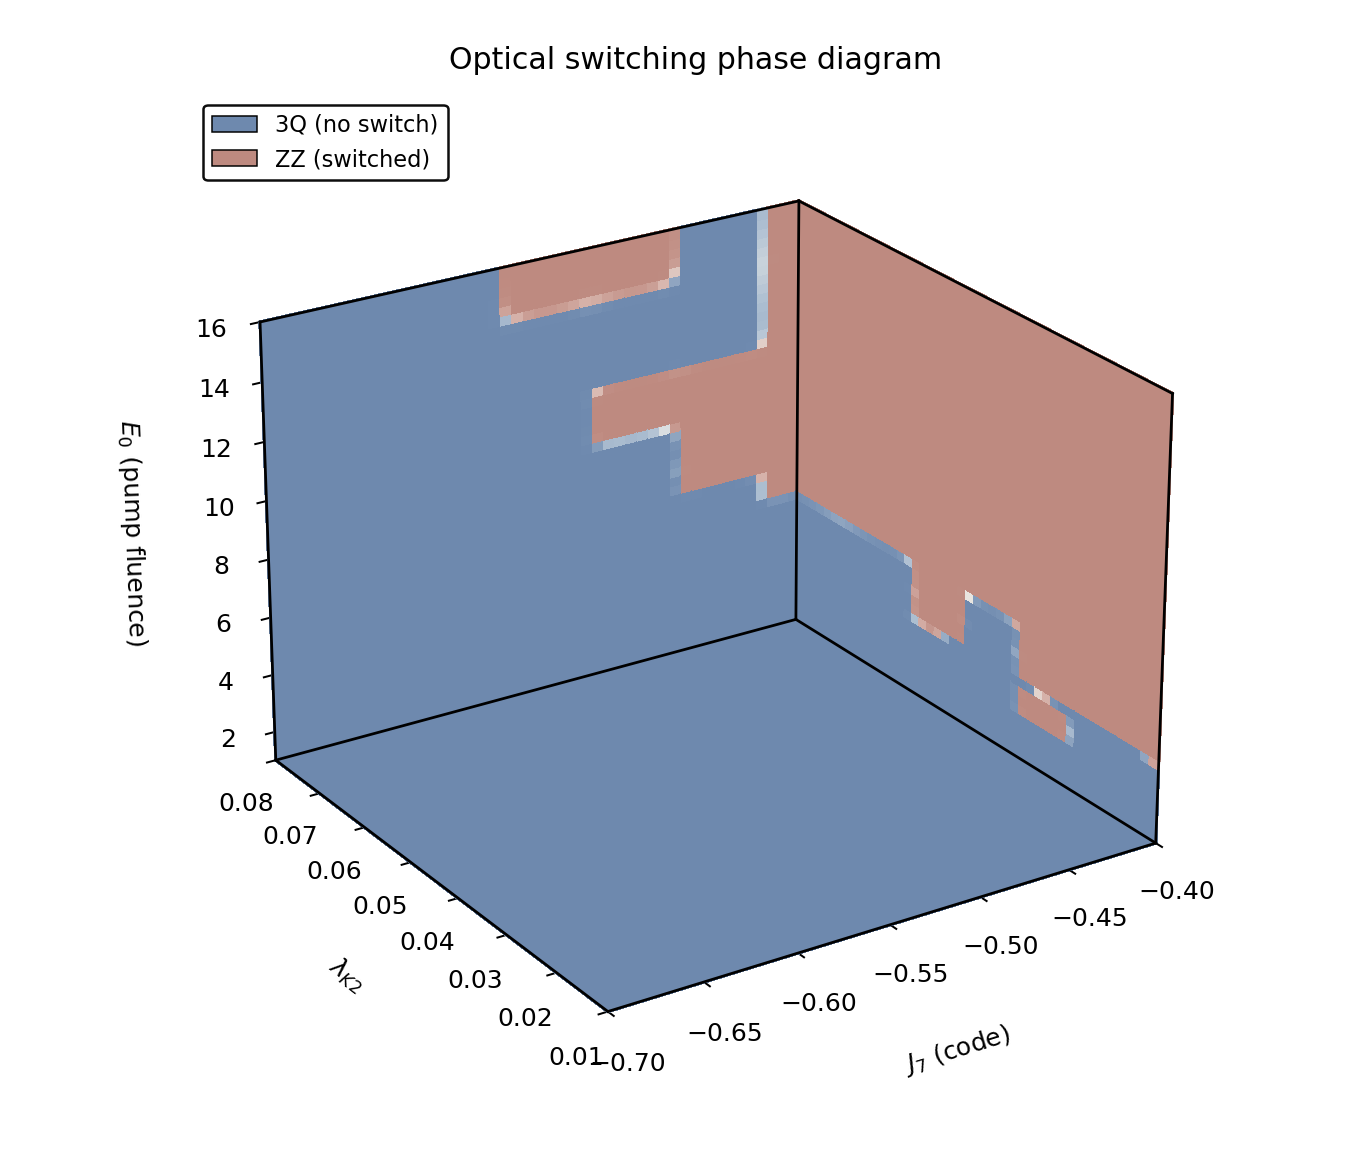
\includegraphics[width=0.98\columnwidth]{figs/cube_phase_diagram.png}
\caption{Clean driven phase diagram at the tuned-Kruger point.  The clean system
is the control problem: it has a comparatively sharp threshold between a stable
\threeQ{} response and a zigzag-like written state.  This cube fixes the
microscopic switching physics that the large-cell disorder calculations broaden.}
\label{fig:cleancube}
\end{figure}

Figure~\ref{fig:cleancube} is the clean baseline.  It shows why disorder must be
included at all.  The pump can access a zigzag-like basin near the tuned
\threeQ--zigzag competition, but in a clean cell this response is organized by a
threshold.  The experimental switching fraction is smoother than this clean
limit, so the disorder calculation should be judged by whether it broadens the
threshold without making zigzag the equilibrium phase before the pump arrives.

\section{One picture}

\begin{figure*}[t]
\centering
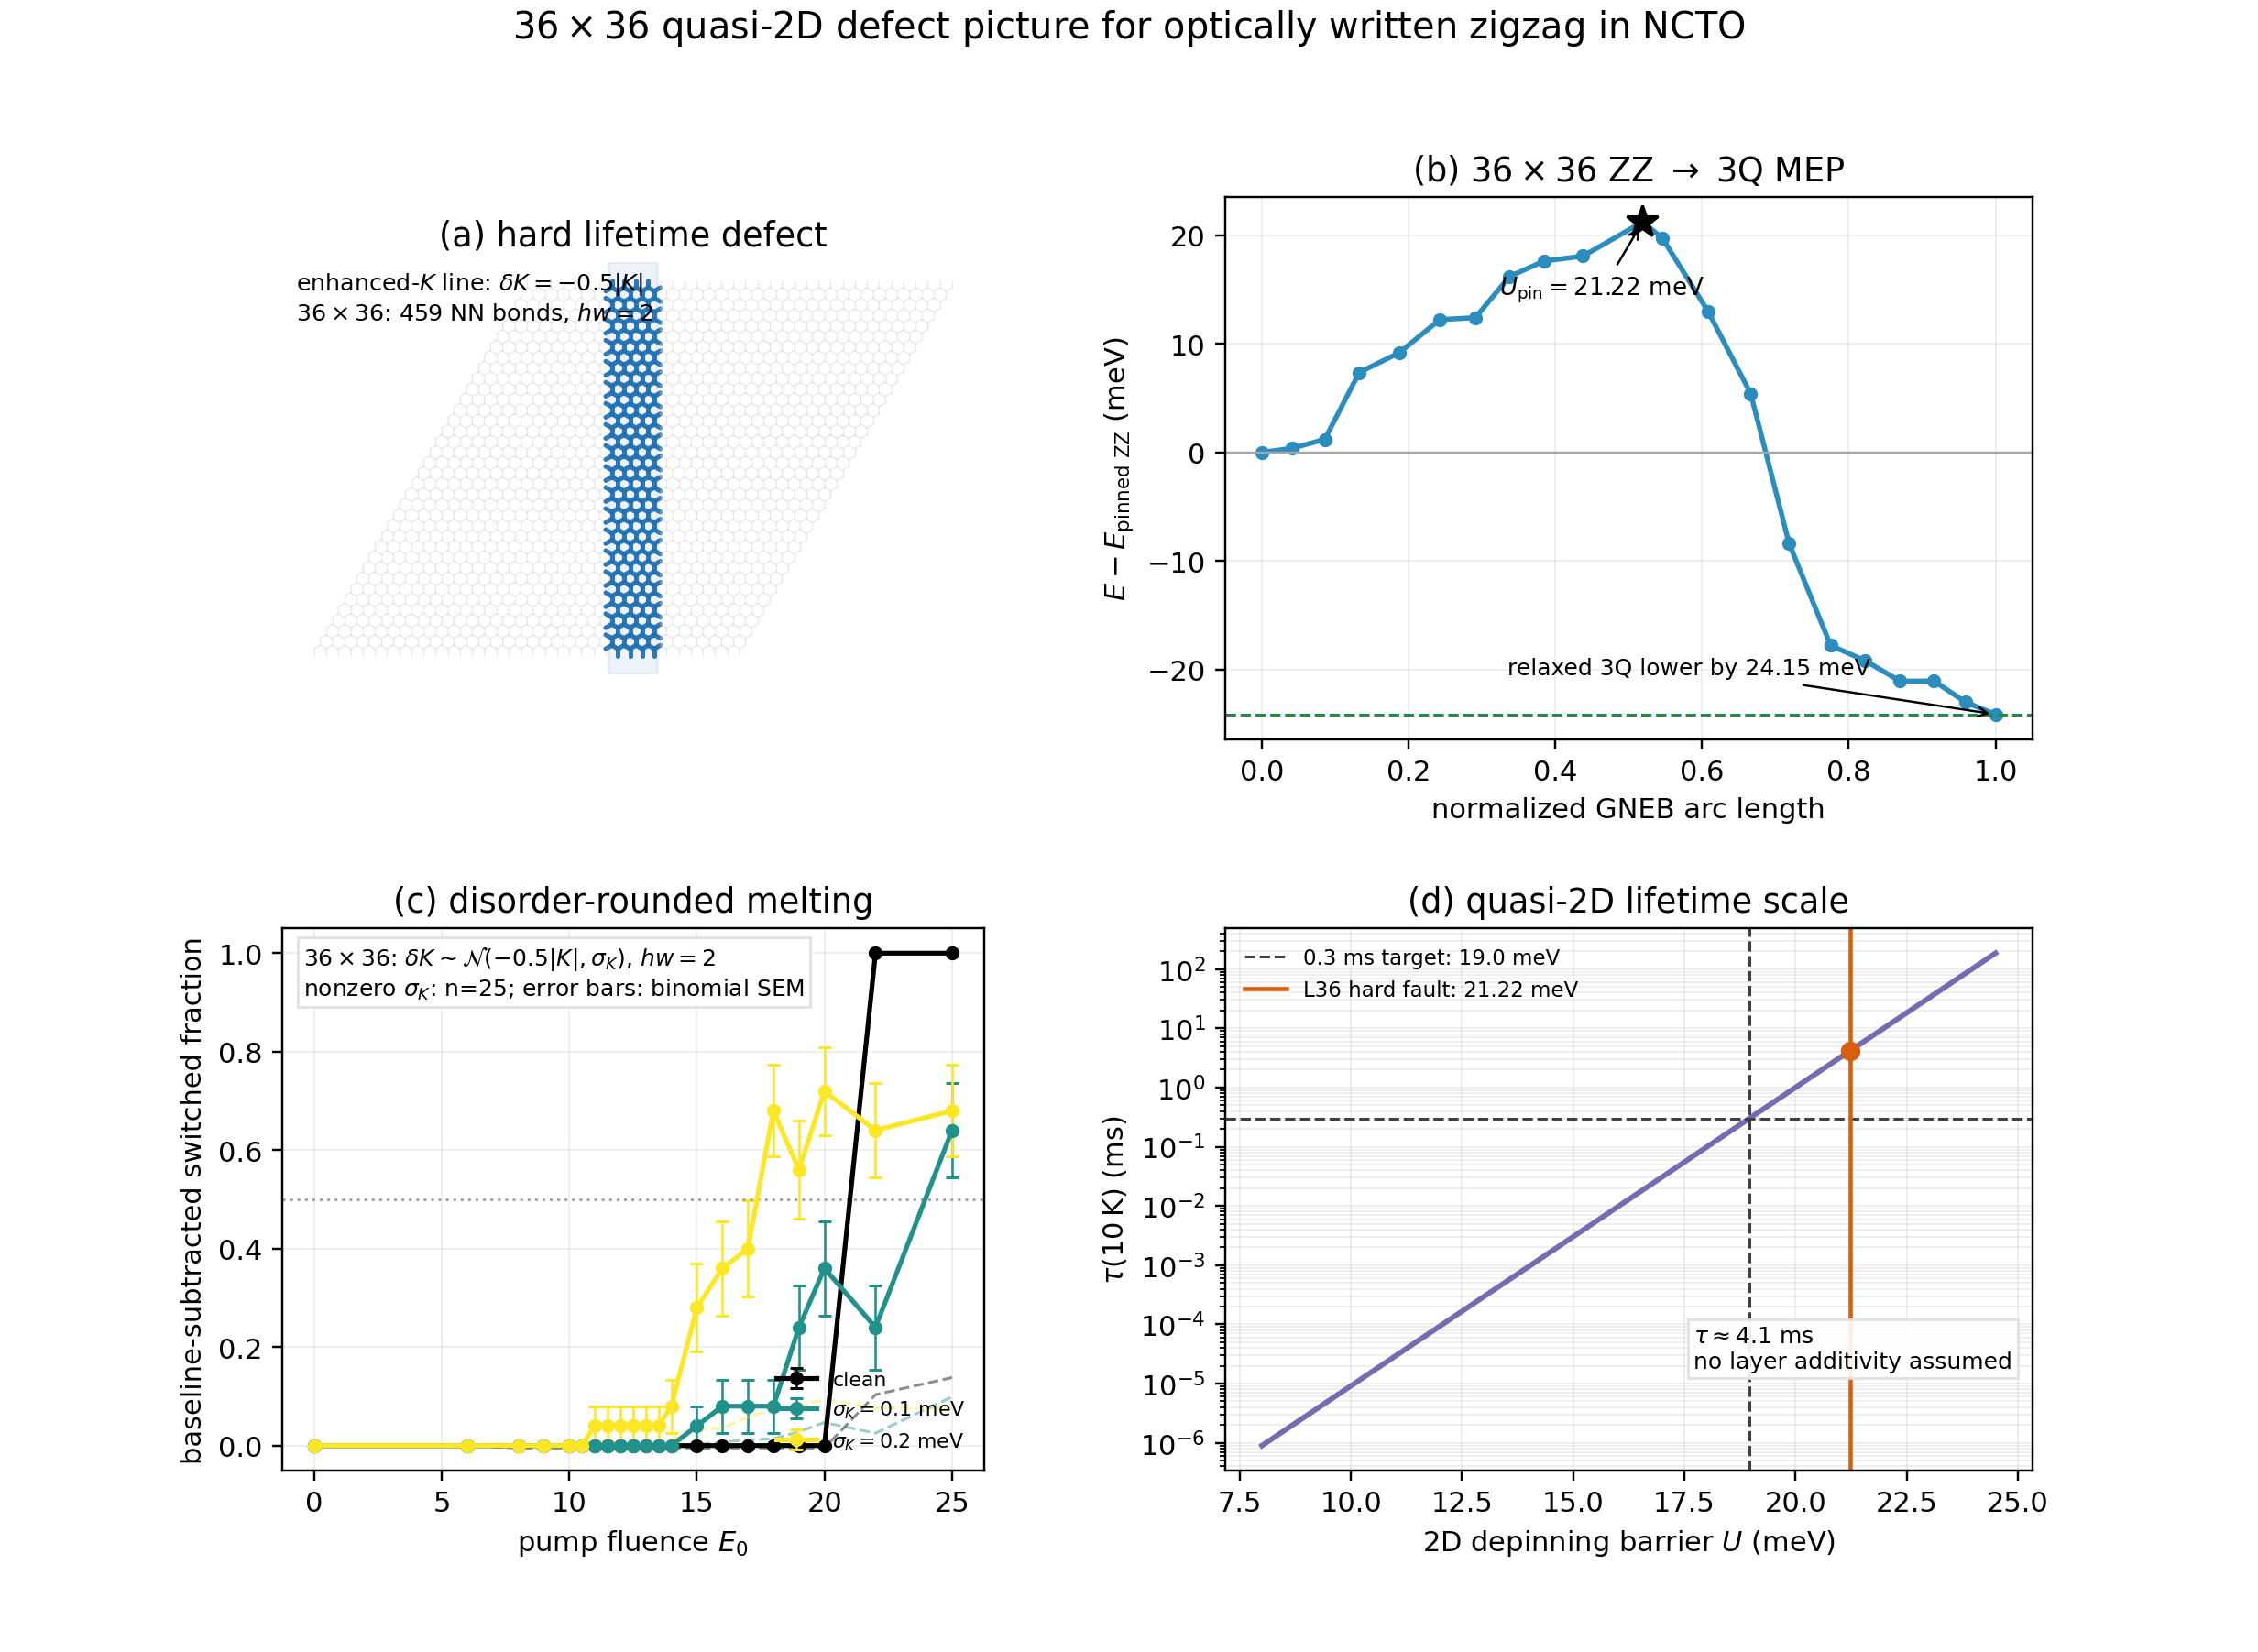
\includegraphics[width=0.98\textwidth]{figs/one_picture_experimental_signatures.png}
\caption{One-defect account of the experimental signatures.  \textbf{(a)} The
hard lifetime defect is an extended line/band of nearest-neighbor bonds on which
the Kitaev magnitude is enhanced: $\delta K=-0.5|K|$, i.e. $K$ is driven more
negative without a sign change.  The selected geometry is a vertical band of
half-width $hw=2$ on the $36\times36$ honeycomb and contains 459 perturbed bonds.
\textbf{(b)} Large-cell GNEB minimum-energy path from pinned zigzag to relaxed
\threeQ{} with this defect present.  The saddle is image 10 and gives
$U_{\rm pin}=21.22\meV$ above the pinned zigzag endpoint; the relaxed \threeQ{}
endpoint lies $24.15\meV$ lower, so the pinned zigzag is metastable, not the
ground state.  \textbf{(c)} The continuous switching/melting signature is
captured on the same $36\times36$ lattice by the same enhanced-$|K|$ line held
fixed at $\delta K_{\rm line}=-0.5|K|$, with zero-mean Gaussian background
$K$ disorder applied to all nearest-neighbor bonds.  Points are baseline-subtracted
switching fractions with binomial standard-error bars; dashed curves are excess
quenched zigzag fractions.  \textbf{(d)} The quasi-two-dimensional Arrhenius
estimate uses the $36\times36$ in-plane depinning barrier directly.}
\label{fig:onepicture}
\end{figure*}

Figure~\ref{fig:onepicture} is the whole proposed mechanism.  The lifetime pin is
not a nematic field and not a smooth random potential.  It is a hard structural
fault: a vertical line/band of nearest-neighbor bonds where the Kitaev exchange
is locally enhanced, $\delta K=-0.5|K|$.  Because $K<0$, this makes $K$ more
negative and increases $|K|$; it does not flip the sign of $K$.  The selected
band has half-width $hw=2$ and covers 459 nearest-neighbor bonds in the
$36\times36$ calculation.  This is the best switchable point in the
extended-defect catalogue: it
has the largest converged depinning barrier among defects for which relaxed
\threeQ{} remains the lower-energy state.

The GNEB panel makes the metastability explicit.  The pinned zigzag endpoint is
the left endpoint and defines zero energy.  The path climbs to
$21.22\meV$ and then descends to the relaxed \threeQ{} endpoint, which is
$24.15\meV$ below pinned zigzag.  Therefore the defect does not make zigzag the
equilibrium phase.  It creates a local trap: zigzag can be written and pinned,
but the surrounding equilibrium order is still \threeQ.  This is exactly the
``switchable'' regime.  The large-cell path ran for 1600 iterations with a stable
saddle image and a last-window barrier scatter of $0.18\meV$, already safely
above the $18.96\meV$ lifetime target.

\begin{figure}[t]
\centering
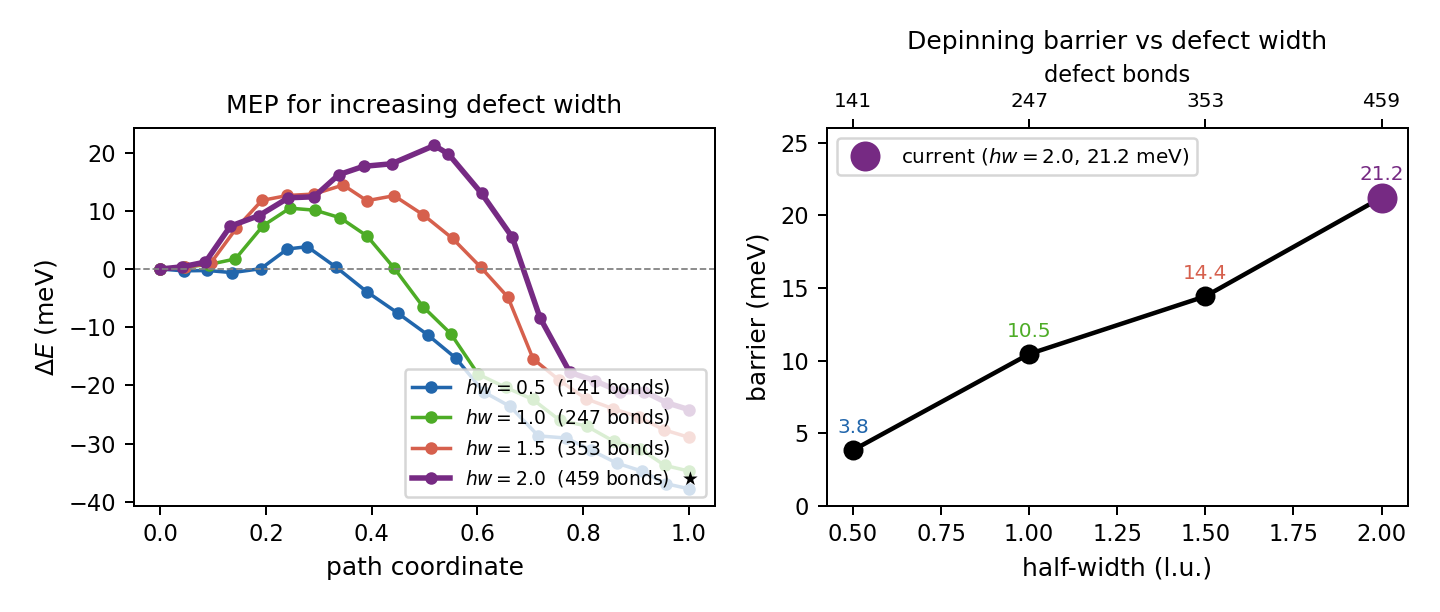
\includegraphics[width=0.98\columnwidth]{figs/selected_kred_mep_L36.png}
\caption{Large-cell hard-fault minimum-energy path on the $36\times36$
honeycomb lattice.  The defect is the same selected enhanced-$|K|$ vertical band,
$\delta K=-0.5|K|$ and $hw=2$, regenerated on the solver lattice.  The path runs
from the pinned zigzag strip to relaxed \threeQ{} with the defect present.  The
barrier is $21.22\meV$, and the relaxed \threeQ{} endpoint is $24.15\meV$ below
the pinned strip, so the written zigzag remains a metastable trapped state.}
\label{fig:l36mep}
\end{figure}

The switching/melting panel uses the same defect family.  The selected line is
kept at the lifetime value $\delta K_{
\rm line}=-0.5|K|$.  To broaden the optical switching fraction we do not vary
the strength of that line; instead we add the earlier zero-mean Gaussian
background disorder to every nearest-neighbor bond,
$\delta K_{\rm bg}\sim\mathcal N(0,\sigma_K)$.  This separates the two roles:
the extended line fixes the hard pinning scale, while the bulk background
inhomogeneity distributes local pump thresholds.  With all-channel coupling the clean fixed-line threshold lies between $E_0=20$
and $22$.  Global disorder lowers and broadens the onset: in the
twenty-five-seed scan, $\sigma_K=0.2\meV$ first shows appreciable switching
above $E_0\simeq14$ and reaches $\sim70\%$ by $E_0=18$--$20$;
$\sigma_K=0.3\meV$ reaches $88\%$ at $E_0=25$ with onset beginning near
$E_0\simeq14$; $\sigma_K=0.5\meV$ shows switching from $E_0=6$ onward,
saturating near $60$--$64\%$.  The normalized-onset 25--75\%
widths are $1.00$, $5.30$, $3.00$, $6.79$, $4.19$, and $5.00$ in $E_0$ for
$\sigma_K=0$, $0.1$, $0.2$, $0.3$, $0.4$, and $0.5\meV$, respectively.  This is the cleanest switching-fraction
cross-check: the line defect is held fixed, and only the background disorder
controls the rounding.

\begin{figure}[t]
\centering
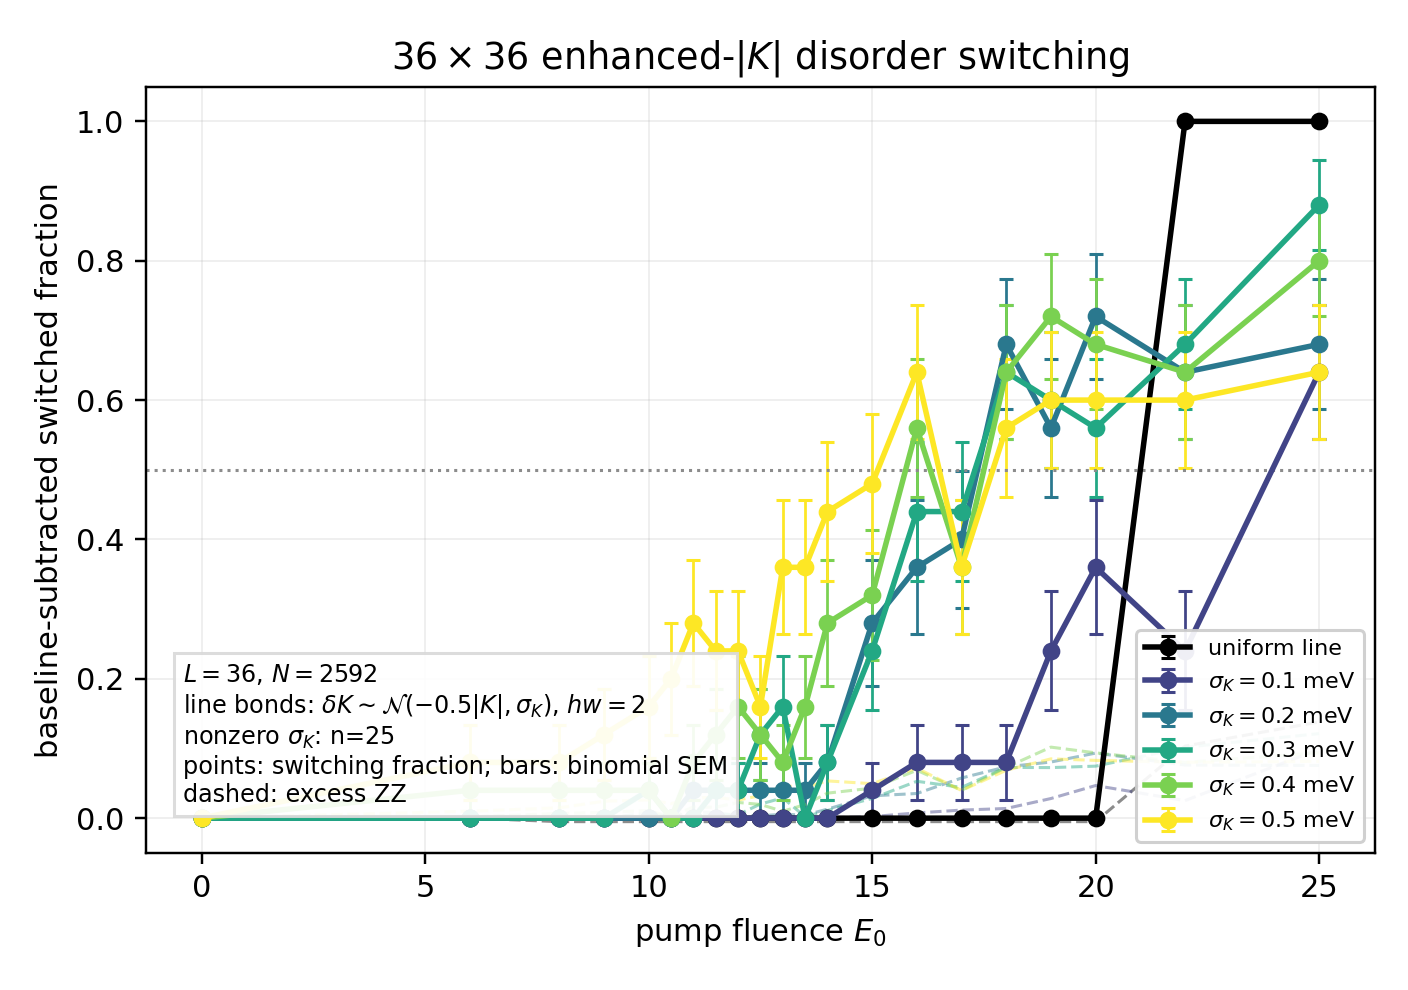
\includegraphics[width=0.98\columnwidth]{figs/l36_switching_rounding.png}
\caption{Large-cell switching-fraction check on a $36\times36$ honeycomb lattice
($N=2592$ spins).  The calculation uses the same enhanced-$|K|$ line as the
lifetime MEP: selected bonds in a $hw=2$ vertical band have the fixed offset
$\delta K_{\rm line}=-0.5|K|$, while all nearest-neighbor bonds also receive
zero-mean background disorder $\delta K_{\rm bg}\sim\mathcal N(0,\sigma_K)$.  All
geometry, reference states, disorder files, driven MD runs, and quenches are
regenerated on the $36\times36$ solver lattice.  The displayed
pump range covers the broadened onset of the fixed-line/global-disorder
protocol.  Nonzero-disorder curves use twenty-five seeds; error bars in
Fig.~\ref{fig:onepicture}(c) denote the binomial standard error of the switching
fraction.}
\label{fig:l36switching}
\end{figure}

\begin{figure}[t]
\centering
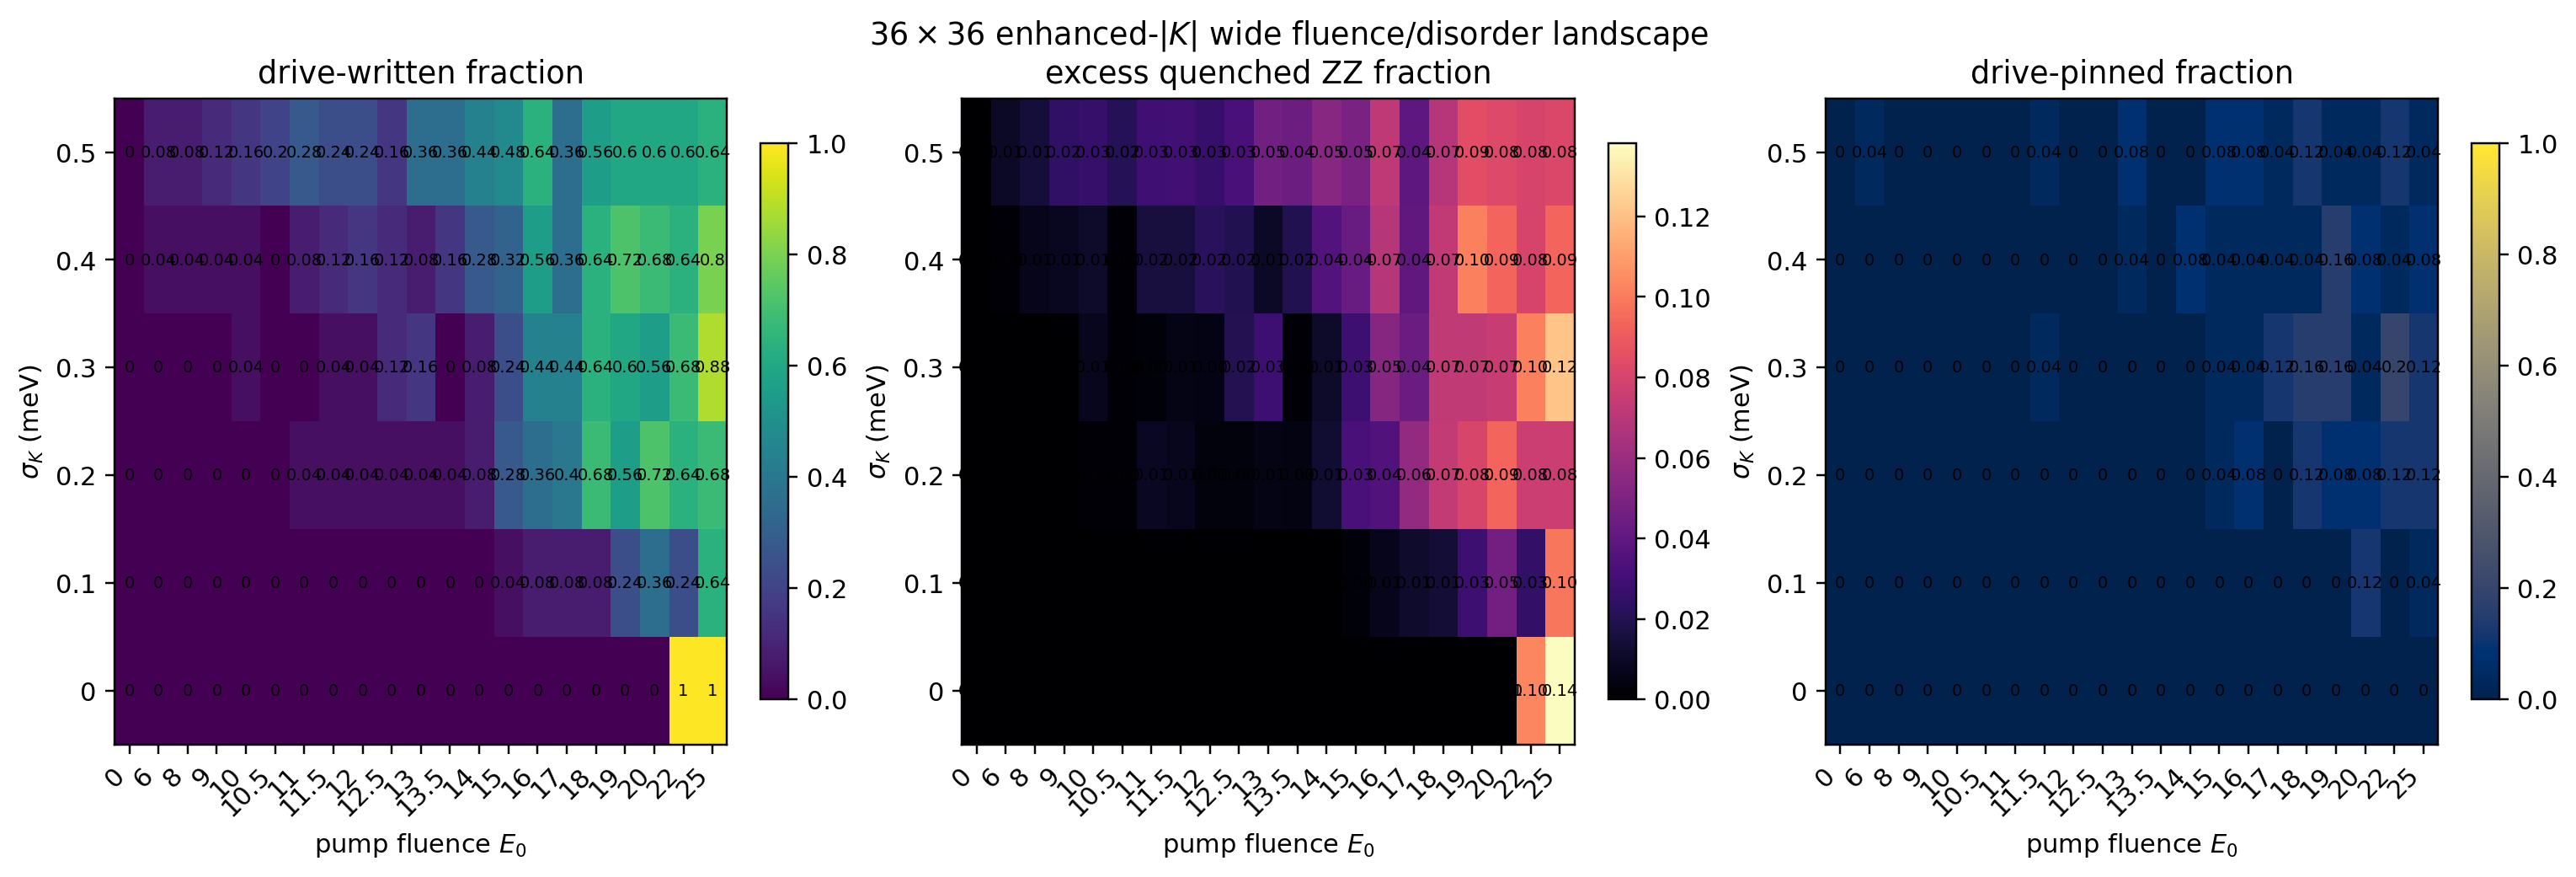
\includegraphics[width=0.98\columnwidth]{figs/l36_switching_wideEwideSigma_heatmap.png}
\caption{Fluence/disorder map for the fixed-line/global-background protocol on
the $36\times36$ lattice.  The enhanced-$|K|$ line is held fixed at
$\delta K_{\rm line}=-0.5|K|$ for every row, while the background Gaussian width
$\sigma_K$ varies across all nearest-neighbor bonds.  The left panel is the
baseline-subtracted drive-written fraction, the middle panel is the excess
quenched zigzag fraction, and the right panel is the pinned-written fraction.}
\label{fig:l36wide}
\end{figure}

\section{Lifetime scale}

The Arrhenius estimate is
\begin{equation}
\tau=\tau_0\exp\left(\frac{U}{k_B T}\right),\qquad
\tau_0=\frac{\hbar}{|K|}=0.0834\,\mathrm{ps}.
\end{equation}
At $T=10$ K, a $0.3$ ms lifetime requires
\begin{equation}
U_{0.3\,\mathrm{ms}}=k_B T\log\left(\frac{0.3\,\mathrm{ms}}{\tau_0}\right)
=18.96\meV.
\end{equation}
The $36\times36$ quasi-two-dimensional hard-fault barrier is $21.22\meV$.  With
the same attempt time this gives $\tau\simeq4.1$ ms at 10 K, above the $0.3$ ms
target.  Since NCTO is treated here as a quasi-two-dimensional magnet, this
in-plane barrier is the lifetime estimate used in the paper.

\section{Other scenarios considered}

The one-picture mechanism is the result of ruling out several cleaner-looking
but less robust explanations.

\paragraph{Clean intrinsic barrier.}
The clean near-degenerate model switches sharply and does not supply a robust
millisecond barrier.  The clean GNEB landscape is too shallow and too spatially
uniform; it can explain a threshold but not a long pinned lifetime.

\paragraph{Classical nucleation theory.}
The CNT droplet language was useful for scale estimates, but it is not the right
story for the observed metastability.  A finite zigzag patch in a clean \threeQ{}
background is not guaranteed to be a stable droplet.  It either shrinks or grows
depending on the local bias and wall motion.  The long lifetime has to come from
boundary depinning at real defects, not from a clean bulk nucleation barrier.

\paragraph{Point defects and vacancies.}
Vacancies or isolated bond defects perturb too few bonds.  They can locally
distort a domain wall, but their depinning barriers remain well below the
$19\meV$ target unless the perturbation becomes so large and extended that it is
no longer a point defect.  Bond-vacancy scans also do not give a clean monotonic
route to a switchable high barrier.

\paragraph{Kitaev sign flip.}
A local $K$ sign flip is a strong microscopic perturbation, but it is not the
best physical candidate.  In the catalogue it does not outperform the enhanced-
$|K|$ fault in the switchable regime, and it is harder to motivate as a modest
structural distortion of the Co--O--Co exchange path.

\paragraph{Nematic fault as the lifetime pin.}
Nematic defects are efficient at selecting zigzag, but this is exactly why they
are dangerous.  A strong nematic bias couples directly to the global zigzag
director and tends to make zigzag the ground state.  That is over-pinning, not a
reversible metastable written state.  We therefore do not use nematic as the
final switching or lifetime defect.

\paragraph{Global zero-mean K disorder.}
The final switching calculation keeps the enhanced-$|K|$ line fixed at
$\delta K_{\rm line}=-0.5|K|$ and adds zero-mean Gaussian disorder
$\delta K_{\rm bg}\sim\mathcal N(0,\sigma_K)$ to every nearest-neighbor bond.
This separates the two roles cleanly: the fixed line controls the hard depinning
scale, while the global bond inhomogeneity distributes local pump thresholds
without introducing a second defect species.

\paragraph{Instantly adiabatic strain along GNEB.}
We do not assume that strain dynamically follows every image during a real pump
trajectory.  The GNEB calculation is a static transition-state calculation for
the spin barrier with the chosen defect present.  The switching simulations are
separate driven dynamical calculations.  This distinction is important: the MEP
establishes the thermal depinning barrier of the written state; it is not meant
to describe the full nonequilibrium phonon-assisted writing process image by
image.

\section{Experimental signatures}

This picture makes four directly checkable claims.  First, samples with more
extended in-plane structural faults should show longer written-state lifetimes,
with an exponential sensitivity to the two-dimensional depinning barrier.  Second,
the written state should remain metastable: after removing the pump, relaxed \threeQ{}
is still the lower-energy state away from the defect.  Third, the optical
switching fraction should broaden continuously as the enhanced-$|K|$ line becomes
spatially inhomogeneous, not jump as a perfectly clean threshold.  In the present
$36\times36$ statistics this appears as fractional switching at the onset
fluences: with $\sigma_K=0.3\meV$ the drive-written fraction rises from $1/4$
around $E_0=8$--$9$ to $3/4$ by $E_0=10.5$.  Fourth, the
lifetime and the switching width probe different aspects of the same fault
family: the mean offset controls the depinning barrier, while the width of the
bond-offset distribution controls the threshold distribution.

The resulting story is deliberately narrow.  A hard enhanced-K structural line
fault pins the boundary and gives a converged ZZ-to-3Q depinning barrier.  The
same line, with Gaussian bond-to-bond variation around $\delta K=-0.5|K|$,
broadens the optical threshold into a fractional seed-resolved onset.  Together they reconcile the sharp lifetime
signature with continuous magnetic melting without making zigzag the equilibrium
state.

\begin{thebibliography}{9}

\bibitem{Bessarab2015}
P.~F.~Bessarab, V.~M.~Uzdin, and H.~Jonsson,
\textit{Method for finding mechanism and activation energy of magnetic
transitions, applied to skyrmion and antivortex annihilation},
Comput. Phys. Commun. \textbf{196}, 335 (2015).

\bibitem{Henkelman2000}
G.~Henkelman, B.~P.~Uberuaga, and H.~Jonsson,
\textit{A climbing image nudged elastic band method for finding saddle points
and minimum energy paths},
J. Chem. Phys. \textbf{113}, 9901 (2000).

\bibitem{Songvilay2020}
M.~Songvilay \emph{et al.},
\textit{Kitaev interactions in the Co honeycomb antiferromagnets
Na$_3$Co$_2$SbO$_6$ and Na$_2$Co$_2$TeO$_6$},
Phys. Rev. B \textbf{102}, 224429 (2020).

\bibitem{Lefrancois2016}
E.~Lefrancois \emph{et al.},
\textit{Magnetic properties of the honeycomb oxide Na$_2$Co$_2$TeO$_6$},
Phys. Rev. B \textbf{94}, 214416 (2016).

\bibitem{Winter2016}
S.~M.~Winter, Y.~Li, H.~O.~Jeschke, and R.~Valenti,
\textit{Challenges in design of Kitaev materials: Magnetic interactions from
competing energy scales},
Phys. Rev. B \textbf{93}, 214431 (2016).

\end{thebibliography}

\end{document}
